\documentclass[12pt, a4paper]{report}
\usepackage{graphicx}
\usepackage{amsmath}
\usepackage{float}
\renewcommand{\baselinestretch}{1.2} 
\usepackage{ragged2e}
\usepackage{fancyvrb}
\usepackage{amssymb}
\usepackage[a4paper, total={7in, 9in}]{geometry}
\usepackage[utf8]{inputenc}
\usepackage{physics}

\begin{document}		
\title{\textbf{EE2703 : Applied Programming Lab \\ Assignment 7 \\ Laplace Transformation}} % Title
\author{Adityan C G EE19B003} % Author name
\date{April 2021} % Date for the report
\maketitle % Insert the title, author and date

\section*{Introduction}
In this assignment, we will look at how to analyse “Linear Time-invariant Systems”with numerical tools in Python.  LTI systems are what Electrical Engineers spend most of their time thinking about - linear circuit analysis or communication channels for example.In this assignment we will use mostly mechanical examples, but will move on to circuits in the next assignment.All the problems will be in “continuous time” and will use Laplace Transforms. Python has  a  Signals  toolbox  which  is  very  useful  and  complete.

\begin{itemize}
  	\item Analysis of continuous time LTI systems in laplace domain through python libraries
    \item Solve \textbf{LCCDE - Linear Constant Coefficient Differential Equations} in laplace  domain using the \texttt{signal} toolbox of \texttt{scipy} library.
  	\item Explore various functions of the above mentioned library like \texttt{impulse, bode, lti, lsim}
\end{itemize}

\section*{Problem 1 and 2}
The time response of a lossless spring system is given by
\begin{equation*}
\ddot{x}(t) + 2.25x(t) = f(t)
\end{equation*}
where $f(t)$ is the forced input on the spring system.
Suppose if the forced input $f(t)$ is a decaying sinusoidal force as given by
\begin{equation*}
f(t) = cos(1.5t)e^{-0.5t}u(t)\\
\end{equation*}
\begin{equation*}
F(s) = \frac{s + 0.5}{(s+0.5)^2 + 2.25}\\
\end{equation*}
with $x(0) = 0$ and $\dot{x} = 0$ input conditions. This corresponds to 
\begin{equation*}
s^2X(s) + 2.25X(s) = F(s)\\
\end{equation*}
\begin{equation*}
H(s) = s^2 + 2.25 = \frac{F(s)}{X(s)}\\
\end{equation*}
\begin{equation*}
X(s) = \frac{s+0.5}{(s^2 + 2.25)((s+0.5)^2 + 2.25)}\\
\end{equation*}

When the damping coefficient is 0.05
\begin{equation*}
f(t) = cos(1.5t)e^{-0.05t}u(t)\\
\end{equation*}
\begin{equation*}
F(s) = \frac{s + 0.05}{(s+0.05)^2 + 2.25}\\
\end{equation*}
\begin{equation*}
X(s) = \frac{s+0.5}{(s^2 + 2.25)((s+0.5)^2 + 2.25)}\\
\end{equation*}

\clearpage
We try to find the time domain form of $X(s)$ using the \texttt{impulse} function
(\texttt{a} is the decay coefficient)
\begin{verbatim}
Time vector going from 0 to 50 seconds 
t = np.linspace(0,50,1000)

X = sp.lti([1, a],np.polymul([1,0,2.25], np.polyadd(np.polymul([1, a],[1, a]),[2.25])))

t, x = sp.impulse(X, None, t)
\end{verbatim}

\begin{center}
	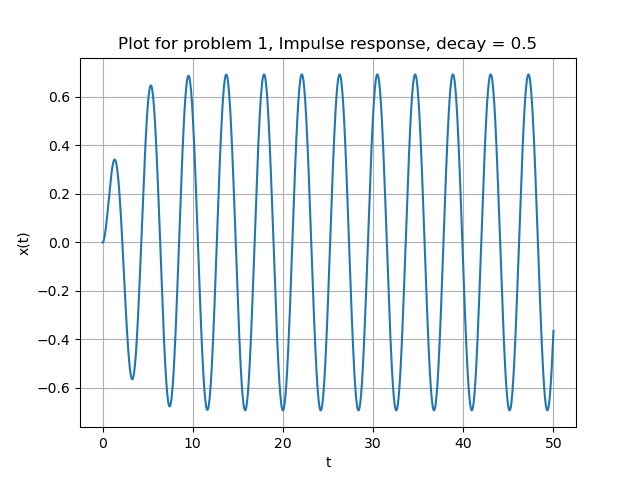
\includegraphics[scale=0.8]{Figure_1.png} 
	\caption{\\X(t) in time domain for decay coefficient 0.5}
	\label{fig:rawdata}
\end{center}

\begin{itemize}
     \item The output of the system when the decay coefficient = 0.05 (in the next graph) has higher amplitude - since the energy supplied by the forced input in case of decay coefficient = 0.05 will be higher compared to decay coefficient = 0.5 as the former one decays slower compared to the second one.
\end{itemize}

\begin{center}
	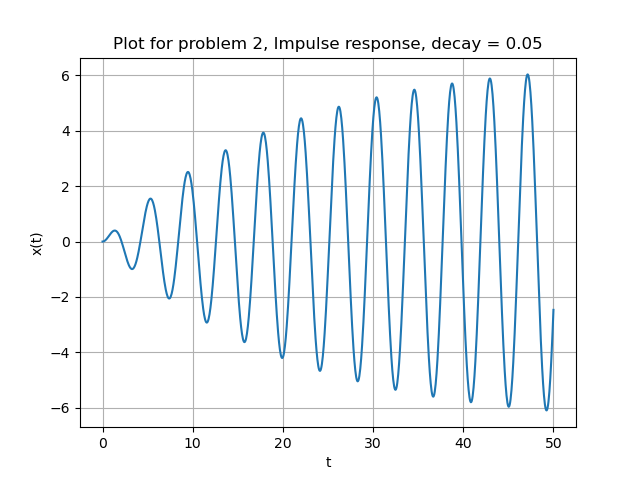
\includegraphics[scale=0.8]{Figure_2.png} 
	\caption{\\X(t) in time domain for decay coefficient 0.05}
	\label{fig:rawdata}
\end{center}

\section*{Problem 3}
We can also notice this while plotting the output for various frequencies. The output with frequency 1.5 rad/s corresponds to the maximum amplitude .
\begin{itemize}
     \item Suppose if the decay coefficient = 0, then the forced input with oscillation frequency $\omega = 1.5$ resonates with the natural frequency of the system thus blowing up the output. 
     \item \textbf{This because the frequency response $H(j\omega)$ has a double pole at $\omega = 1.5$}
\end{itemize}
\begin{center}
	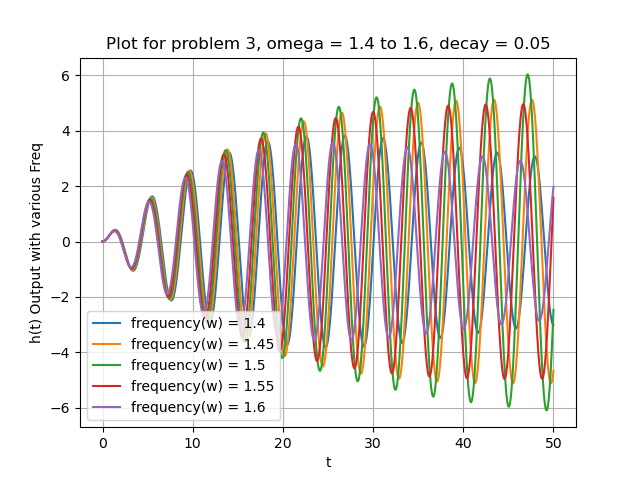
\includegraphics[scale=0.8]{Figure_3.png} 
	\label{fig:rawdata}
\end{center}


\section*{Problem 4}
We try to solve the following coupled spring problem with:
\begin{equation*}
\ddot{x} + (x-y) = 0
\end{equation*}
\begin{equation*}
\ddot{y} + 2(y-x) = 0
\end{equation*}
with initial conditions $x(0) = 1$, $\dot{x}(0) = y(0) = \dot{y}(0) = 0$. Solving further 
\begin{equation*}
s^2X(s) -sx(0^-) - \dot{x}(0^-) = Y(s)
\end{equation*}
\begin{equation*}
s^2Y(s) -sy(0^-) - \dot{y}(0^-) + 2Y(s)= X(s)
\end{equation*}
Substituting and solving further, we arrive at
\begin{equation*}
X(s) = \frac{(0.5s^2+1)s}{(s^2 + 1)(0.5s^2 + 1) - 1}\\
\end{equation*}
\begin{equation*}
Y(s) = \frac{s}{(s^2 + 1)(0.5s^2 + 1) - 1}\\
\end{equation*}

\begin{verbatim}
t = np.linspace(0, 20, 1000)

X = sp.lti(np.polymul([1, 0], [0.5, 0, 1]), np.polyadd(np.polymul([1, 0, 1], [0.5, 0, 1]), [-1]))
Y = sp.lti([1, 0], np.polyadd(np.polymul([1, 0, 1], [0.5, 0, 1]), [-1]))

t, x = sp.impulse(X, None, t)
t, y = sp.impulse(Y, None, t)
\end{verbatim}

\begin{center}
	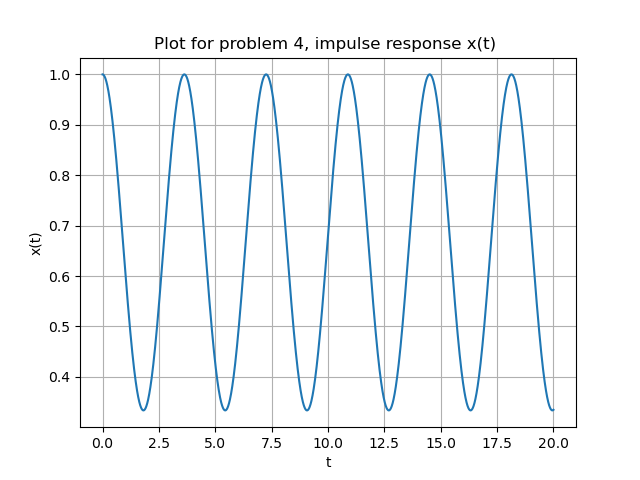
\includegraphics[scale=0.8]{4a.png} 
	\label{fig:rawdata}
\end{center}
\begin{center}
	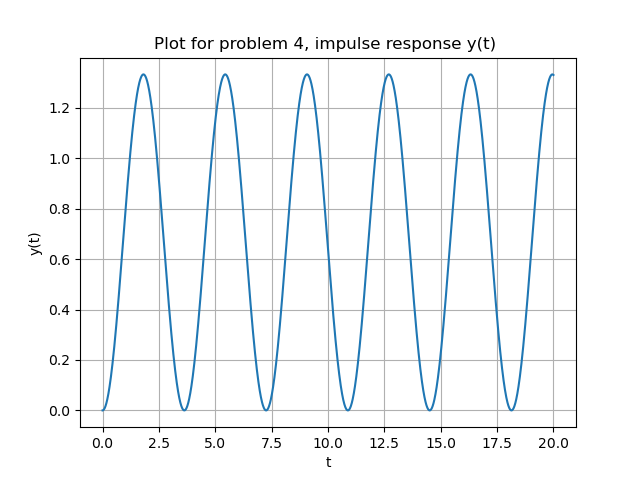
\includegraphics[scale=0.8]{4b.png} 
	\label{fig:rawdata}
\end{center}

\section*{Problem 5}
The next part of the problem is to obtain the magnitude and phase response of the steady state transfer function of the RLC Circuit. We can observe that the circuit acts as a voltage divider. Thus it reduces to the following transfer equation
\begin{equation*}
H(s) = \frac{1}{1 + RCs + LCs^2} = \frac{1}{1 + 10^{-4}s + 10^{-12}s^2}\\
\end{equation*}

\begin{verbatim}
H = sp.lti([1], [1e-12, 1e-4, 1])
w, S, phi = H.bode()
\end{verbatim}

\begin{center}
	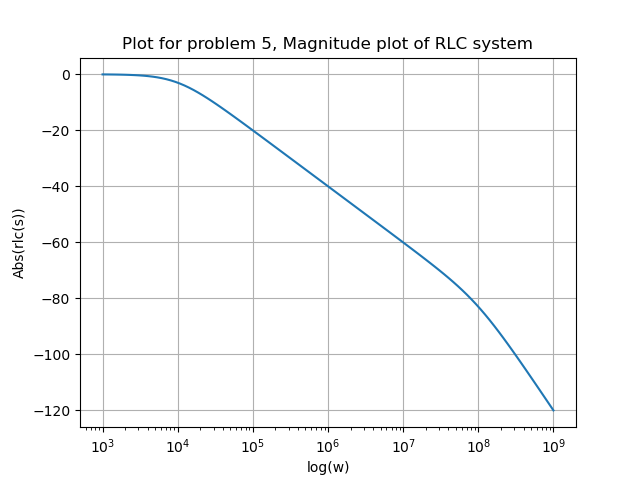
\includegraphics[scale=0.8]{5a.png} 
	\label{fig:rawdata}
\end{center}

\begin{center}
	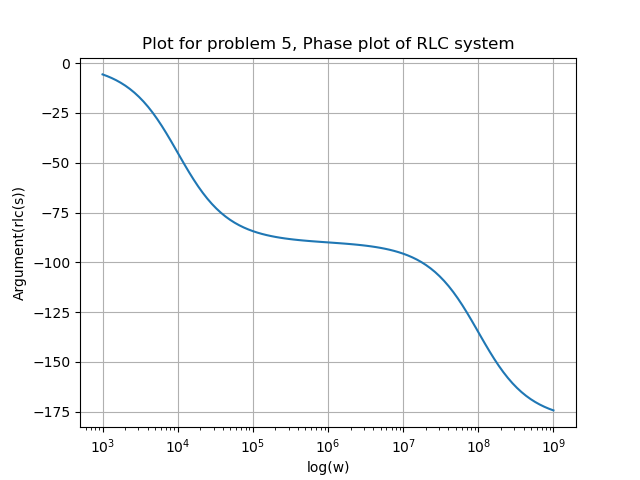
\includegraphics[scale=0.8]{5b.png} 
	\label{fig:rawdata}
\end{center}

 In the magnitude plot remains constant until it sees a pole after which it decreases rapidly at -20 dB/decade. It further sloped down to -40 dB/decade after it encounters the second pole. 
 In the phase plot, we can observe that there is a phase drop of approximately 90 degrees at each pole.


\section*{Problem 6}
In the given circuit, if the applied input voltage is of form, 
\begin{equation*}
V_{in}(t) = cos(10^3t)u(t) - cos(10^6t)u(t)
\end{equation*}
We obtain the final output $V_{out}$ of the RLC circuit by

\begin{verbatim}
Initial short term response :
t_rlc = np.arange(0,30e-6,1e-8)
v_i_st = np.cos(1e3*t_rlc) - np.cos(1e6*t_rlc)
Long term Response :
t_rlc_2 = np.arange(0,0.01,1e-7)
v_i_lt = np.cos(1e3*t_rlc_2) - np.cos(1e6*t_rlc_2)
\end{verbatim}

\begin{center}
	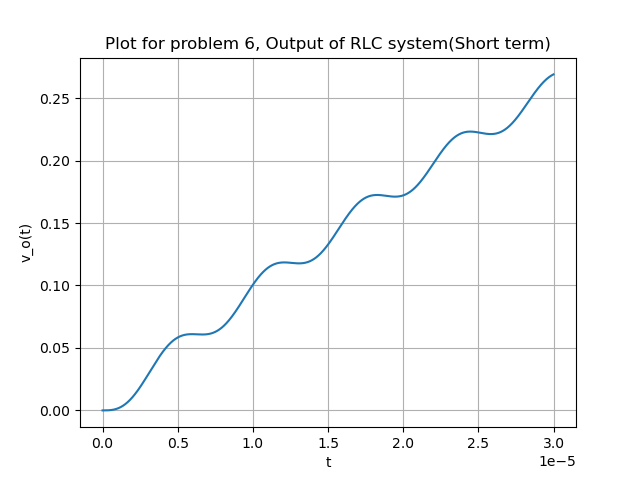
\includegraphics[scale=0.8]{6a.png} 
	\label{fig:rawdata}
\end{center}
The above graph corresponds to the initial transient response of the system. We can observe that the sinusoidal component \texttt{cos(1e6t)} is showed up as ups and downs in the graph.  
\begin{center}
	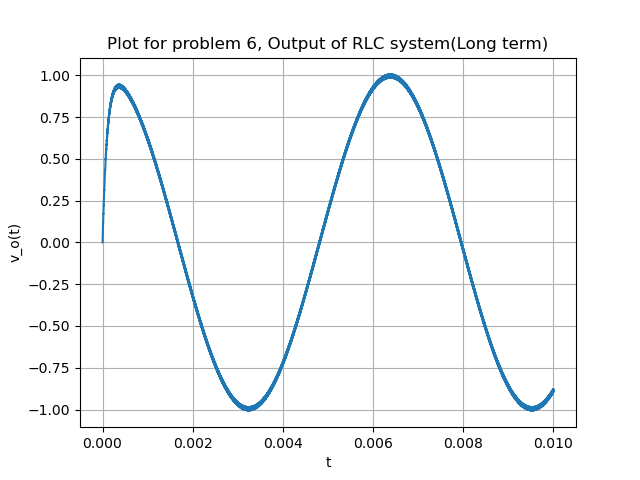
\includegraphics[scale=0.8]{6b.png} 
	\label{fig:rawdata}
\end{center}
But in steady state, we can observe that the output is primarily composed of $1000$ rad/s frequency while the frequency $10^6$ rad/s is almost attenuated. This is because the later frequency experiences attenuation of about $100$ times as shown in the magnitude plot of the transfer function. Essentially the given circuit acts as a low pass filter supporting frequencies upto $1000$ rad/s. 

\section*{Conclusion}
In this assignment, we explored the idea of solving laplace equations of various systems like spring system, coupled spring problem and a RLC system using the \texttt{signal} toolbox of the \texttt{scipy} python library. We observed that when the forced input operates at a frequency close to the natural frequency it resonates with the output. We also observed how a RLC circuit can be used as a low pass filter.

\end{document}

